\documentclass[10pt]{article}
%\documentclass[twoside,leqno,twocolumn]{article}

% Comment out the line below if using A4 paper size
\usepackage[letterpaper]{geometry}

\usepackage{algorithm}
\usepackage{physics}
\usepackage[algo2e,ruled,vlined,linesnumbered]{algorithm2e}
\usepackage{booktabs}

\usepackage{multirow}
\usepackage{longtable}
\usepackage{numprint}
%\usepackage{fullpage}
%\usepackage{multicol}
%\usepackage{wrapfig}
%\usepackage[sort&compress, sectionbib]{natbib}

\usepackage{lipsum}

\usepackage{amsmath}
\usepackage{amsfonts}
\usepackage{mathtools}

\usepackage{hyperref}
\usepackage[usenames,dvipsnames]{xcolor}
\usepackage[normalem]{ulem}
\usepackage[]{graphicx}\usepackage[]{color}
%% maxwidth is the original width if it is less than linewidth
%% otherwise use linewidth (to make sure the graphics do not exceed the margin)
\makeatletter
\def\maxwidth{ %
  \ifdim\Gin@nat@width>\linewidth
    \linewidth
  \else
    \Gin@nat@width
  \fi
}
\makeatother

%\definecolor{fgcolor}{rgb}{0.345, 0.345, 0.345}
%\newcommand{\hlnum}[1]{\textcolor[rgb]{0.686,0.059,0.569}{#1}}%
%\newcommand{\hlstr}[1]{\textcolor[rgb]{0.192,0.494,0.8}{#1}}%
%\newcommand{\hlcom}[1]{\textcolor[rgb]{0.678,0.584,0.686}{\textit{#1}}}%
%\newcommand{\hlopt}[1]{\textcolor[rgb]{0,0,0}{#1}}%
%\newcommand{\hlstd}[1]{\textcolor[rgb]{0.345,0.345,0.345}{#1}}%
%\newcommand{\hlkwa}[1]{\textcolor[rgb]{0.161,0.373,0.58}{\textbf{#1}}}%
%\newcommand{\hlkwb}[1]{\textcolor[rgb]{0.69,0.353,0.396}{#1}}%
%\newcommand{\hlkwc}[1]{\textcolor[rgb]{0.333,0.667,0.333}{#1}}%
%\newcommand{\hlkwd}[1]{\textcolor[rgb]{0.737,0.353,0.396}{\textbf{#1}}}%
%\let\hlipl\hlkwb
%\def\MdR{\ensuremath{\mathbb{R}}}
%\def\MdN{\ensuremath{\mathbb{N}}}

% fixing lines ending on one word etc...
\setlength\parfillskip{0pt plus .4\textwidth}
\setlength\emergencystretch{.1\textwidth}
\clubpenalty10000
\widowpenalty10000
\displaywidowpenalty=10000

%\usepackage{framed}
%\makeatletter
%\newenvironment{kframe}{%
% \def\at@end@of@kframe{}%
% \ifinner\ifhmode%
%  \def\at@end@of@kframe{\end{minipage}}%
%  \begin{minipage}{\columnwidth}%
% \fi\fi%
% \def\FrameCommand##1{\hskip\@totalleftmargin \hskip-\fboxsep
% \colorbox{shadecolor}{##1}\hskip-\fboxsep
%     % There is no \\@totalrightmargin, so:
%     \hskip-\linewidth \hskip-\@totalleftmargin \hskip\columnwidth}%
% \MakeFramed {\advance\hsize-\width
%   \@totalleftmargin\z@ \linewidth\hsize
%   \@setminipage}}%
% {\par\unskip\endMakeFramed%
% \at@end@of@kframe}
%\makeatother

%\definecolor{shadecolor}{rgb}{.97, .97, .97}
%\definecolor{messagecolor}{rgb}{0, 0, 0}
%\definecolor{warningcolor}{rgb}{1, 0, 1}
%\definecolor{errorcolor}{rgb}{1, 0, 0}
%\newenvironment{knitrout}{}{} % an empty environment to be redefined in TeX

%\usepackage{alltt}
%\newcommand{\SweaveOpts}[1]{}  % do not interfere with LaTeX
%\newcommand{\SweaveInput}[1]{} % because they are not real TeX commands
%\newcommand{\Sexpr}[1]{}       % will only be parsed by R

\newcommand{\Ciso}{$^{13}$C~}

\newcommand{\ie}{i.e.~}
\newcommand{\etal}{et~al.~}
\newcommand{\eg}{e.g.~}
\newcommand{\wolog}{w.l.o.g.~}
\newcommand{\wrt}{w.r.t.~}
\newcommand{\cf}{cf.~}

\newcommand{\mb}[1]{\mathbf{#1}}
\DeclareMathOperator\nullity{\mathrm{nullity}}
\DeclareMathOperator\Reals{\mathbb{R}}
\let\Pr\relax
\DeclareMathOperator\Pr{\mathbb{P}}
\DeclareMathOperator\tk{\mathcal{T}}
\DeclareMathOperator\is{\mathcal{I}}
\DeclareMathOperator\fp{\mathcal{V}}
\DeclareMathOperator\ffp{\mathcal{\hat{V}}}
\DeclareMathOperator\likeli{\ell}
%\DeclareMathOperator\ssr{\mathrm{SSR}}
\DeclareMathOperator\supp{\mathrm{supp}}
\DeclareMathOperator\bmu{\boldsymbol{\mu}}
\DeclareMathOperator\bomega{\boldsymbol{\omega}}

\newcommand{\todo}[1]{{\color{red}#1}}

\usepackage{capt-of}%
\usepackage{caption}
\usepackage{xspace}

\usepackage{etoolbox}
%\usepackage[left,pagewise] {lineno}
%\definecolor {infocolor} {rgb} {0.6,0.6,0.6}
%\renewcommand\linenumberfont{\normalfont\normalsize\textcolor{infocolor}}
%\linenumbers

%\bibliographystyle{plainurl}
%\patchcmd{\thebibliography}{\list}{\fontsize{0.98em}{0.9\baselineskip}\selectfont\list}{}{} 

% \renewcommand{\ssch}[1]{}

%\newcommand{\mytitle}{\textsc{Improving Sampling Efficiency in \Ciso Metabolic Flux Analysis}}
\newcommand{\mytitle}{\textsc{Improving Efficiency of Markov \\ Chain Monte Carlo Algorithms for \Ciso Metabolic Flux Analysis}}
\newcommand{\mysubtitle}{\textsc{Master Thesis Expos\'e}}

\begin{document}
    \begin{titlepage}
	\centering
	\phantom{hello}
	\vspace{2cm}
	{\scshape\Large University of Vienna\par}
	\vspace{0.1cm}
	{\scshape\LARGE Master Thesis Expos\'e \par}
	%{\scshape\LARGE University of Vienna\par}
	%\vspace{0.2cm}
	%{\scshape\Large Master Thesis Expos\'e \par}
	\vspace{1cm}
	%{\scshape\huge\bfseries Improving Efficiency of Markov Chain Monte Carlo Algorithms for \Ciso Metabolic Flux Analysis \par}
	{\scshape\huge Improving Efficiency of Markov Chain Monte Carlo Algorithms for \Ciso Metabolic Flux Analysis \par}
	\vspace{1.5cm}
	{\Large Richard D. Paul\par}
	\vspace{0.2cm}
	{\today\par}
	\vspace{2cm}
	\begin{abstract}
	    %\noindent \todo{yet to come} 
	    \noindent \lipsum[1-2]
	\end{abstract}
	\vfill
    \end{titlepage}
%\title{\Large \mysubtitle \\ \vspace{1mm} \huge \mytitle}
%\author{Richard D. Paul}%\thanks{University of Vienna, Faculty of Physics}}
%
%\date{}
%
%\maketitle
%
%\begin{abstract}
%    \noindent \todo{yet to come}
%\end{abstract}

\pagebreak

\section{Introduction}
\label{sec:introduction}

In the field of Metabolomics, Metabolic Flux Analysis (MFA) deals with determining reaction rates in metabolic reaction networks \cite{noeh15}.
A metabolic reaction network maps what substrates get turned over into which metabolites. 
Naively, such a reaction network contains only static information like stoichiometry and possible pathways,
but does not contain any dynamic information, \ie we do not know which reactions happen at what rate or if they happen at all.
Figuratively speaking, if we were to feed an organism with some substrate, then we do not expect all products to be there immediately, 
but instead they get slowly turned over.
Also, depending on the substrate and the external stress that we apply on the organism, we do expect the metabolism to behave differently.
For example, under certain conditions \textit{Aspergillus nidulans} does start emitting toxins when experiencing nutrient depletion \todo{\cite{?}}. 
%In that sense, Metabolic Flux Analysis quantifies the phenotype 

\subsection{An overview}

Measuring reaction rates, to which we will from now on refer to as \emph{fluxes}, directly is in
general only possible for extracellular fluxes like substrate uptake, CO$_2$ production 
or biomass growth. 
For all other fluxes, it is necessary to infer their values from measurement data.
A naming property of \Ciso MFA is to obtain such measurement data from \Ciso isotope labelling 
experiments.
The input substrate gets labelled with \Ciso atoms at predetermined postitions and by time 
labellings will be distributed over the metabolites.
The labellings later can then be measured using nuclear magnetic resonance (NMR) and mass 
spectrometry (MS).
In order to be able to use the isotope labelling experiment data, we need so called atom 
transition networks.
Basic reaction networks usually map molecules to other molecules. 
Atom transition networks concretize reactions on an atomic level, mapping the single atoms of 
the substrate molecule to the atoms in the product molecule by position.
Given such an atom transition network, an input substrate labelling and a \emph{flux 
distributions}, which is a vector of all fluxes, this allows for forward simulations of 
labelling data and hence for computing residuals to quantify the quality of an estimated 
flux distribution.

Equipped with this residual the problem of determining fluxes becomes an optimization problem,
whose solution is also commonly referred to as the \emph{maximum likelihood estimator}.
Such point estimators however become rather meaningless in the presence of multiple optima 
present in the problem at hand.
Apart from non-uniqueness of the solution, point estimators fail to come up for measurement 
noises and hence it is of great interest to also quantify uncertainities that come with likely
solutions.
A modern and very intuitive approach to obtain such uncertainity quantification is provided 
within the Bayesian Framework, where credible intervals are constituted using the posterior 
distribution of the flux distributions given the measurements.
We will refer to the particular problem of approximately computing the posterior distribution of 
the flux distributions as the \emph{flux estimation problem}.
This posterior distribution can in general be approximated by using Markov chain Monte Carlo 
algorithms.
These algorithms run a Markov chain constructed such that in the limit it produces samples 
proportional to the target distribution we desire to compute. 
In general, Markov chain Monte Carlo algorithms are a well-investigated topic \cite{} with a 
large variety of different known proposal distributions and approaches to tune them, of which we 
will discuss some later in this expos\'e.
A distinguishing feature of the parameter estimation problem in \Ciso Metabolic Flux Analysis is 
the presence of a linearly constrained parameter space, turning it into a convex polytope on 
which standard Markov chain Monte Carlo algorithms may work far from optimal \todo{\cite{?}}.
This has led to the development of proposal distributions which are specialized for working on 
convex polytopes like the Dikin and Vaidya walk samplers \cite{chen17, kannan12}.
A more detailed overview over proposal distributions and also on the general notion of Markov 
chain Monte Carlo algorithms is given within Section \ref{sec:preliminaries}.

\subsection{Intended contributions}

Apart from the challenge of developing sampling algorithms optimized for working on convex 
polytopes, the flux estimation problem suffers from costly forward simulations which are needed 
in the acceptance step of the Markov chain Monte Carlo algorithm.
This leads to a natural interest in highly efficient algorithms, where efficiency may be either 
statiscally or computationally.
A quite naive but promising approach seems to be replacing exact but costly forward simulations 
with rather cheap and fast ones in order to pre-select moves which have a higher acceptance rate,
hence reducing the number of costly evaluations for computing steps, which might be rejected 
anyways.
Methods using such cascades of coarse-to-fine models are known as \emph{Multifidelity methods} 
\cite{efendiev06, peherstorfer18}, but to the best of our knowledge have not yet been applied to 
the field of \Ciso Metabolic Flux Analysis.
A more thorough introduction to this approach will be given in Section \ref{sec:multifidelity}.

In order to apply the Multifidelity idea, the question arises of how to obtain such lower 
accuracy models and what pitfalls one may encounter.
Some different approaches which seem promising will be outlined in Section 
\ref{sec:multifidelity}.
On of these approaches includes reducing the measurement data which for which we seek credible
parameter sets, possibly leading to the kind of cheaper models we aim for.
The key idea behined this approach is that any estimate which is able to explain the complete 
data should also be able to explain only parts of the data.

Another idea is to use regression models of pre-run samples closely following \cite{muller20}.
The obvious problem when fitting approximate models on generated samples is that the samples 
taken from a pre-run have no guarantee to be actually representative of the target function 
if the pre-run did not run until convergence.
However, if it ran until convergence, then the problem at hand is already solved, leaving the 
idea of approximate models superfluous.
The issue might be prevented by introducing a trust criterion based on which we decide whether 
the model fitted on the non-convergent pre-run is safe to use or not.
Distrusting the approximate model we switch back to generate proposals without a low fidelity 
pre-filtering. 

\bigskip \noindent 
The aim of this Master's Thesis is to examine the possibilities of employing Multifidelity 
methods to the flux estimation problem as well as developing and implementing such methods in 
detail.
This shall further lead to the development of guidelines for employing such models based not 
only on experimental but also theoretical considerations.
Of particular interest will be the trust criterion approach as it seems not yet much 
investigated.
Also, M\"uller \etal \cite{muller20}, who proposed this approach, apply it only for computing 
the gradient used in their proposal distribution.
To the best of our knowledge there have been no attempts so far to connect this approach with 
the Multifidelity methods mentioned above.
The proclaimed goal of this work is to considerably accelerate existing sampling methods 
especially for the scenario of isotopically nonstationary measurements, which will be discussed 
in some more detail in Section \ref{sec:forward-simulations}.

\section{Preliminaries}
\label{sec:preliminaries}

In the following section we give a simplified and partly superficial overview on the key 
approaches to model metabolic networks and their reaction rates as well as on the very basics of
Bayesian parameter estimation and Markov chain Monte Carlo algorithms.

%The space of possible fluxes can further be restricted by inequality constraints demanding 
%\eg that some fluxes cannot be larger than preceeding ones or fixing the direction in which the reaction happens.
%Imposing these restrictions defines a convex polytope 
%$$
%    P = \{ x \in \mathbb{R}^n : Ax \leq b \}, \, A \in \mathbb{R}^{m \times n}, b \in \mathbb{R}^{m}
%$$
%in which we search for a satisfying solution.
%A solution in this case is a set of fluxes $x \in \mathbb{R}^n$ from which we can then compute the full flux distribution.

\subsection{Stoichiometric modelling}
\label{sec:stoichiometric-modelling}

The metabolism of an organism is defined by a set of biochemical reactions which turn substrates into energy, proteins, 
lipids and further "building blocks" of the organism, as well as other possibly desired compounds e.g. toxins.
Along so called metabolic pathways different substrates will be turned into new products which then again act as 
substrates for further reactions.
An intuitive way of handling the set of metabolic reactions is via reaction networks.
A \emph{reaction network} forms a directed bipratite graph $G=(M \cup R,E)$ consisting of a node set $M$ 
representing the metabolites, i.e. the chemical compounds included throughout the metabolism, 
a node set $R$ representing the reactions and an edge set $E \subseteq M \times R$ of directed edges, 
i.e. $(v,u) \neq (u,v) \in E$.
An alternative but equivalent way to interpret the reaction network is to regard it as a hypergraph, 
where the node set consists of the metabolites only and the directed hyperedges form the reactions.
The previously described bipartite graph is then called the incidence or Levi graph of the latter.

We introduce some basic concepts by the means of the following exemplary chemical reaction equations 
including three not further specified compounds $A, B, C$ and $D$
\begin{align}
    \begin{array}{r r l}
	R_1: & A + B & \to C \\
	R_2: & C & \to B + D
    \end{array} \label{eq:reaction-eqs}
\end{align}
Its reaction network looks as depictured in Figure \ref{fig:reaction-network}.

\begin{figure}%[ht!]
    \centering
    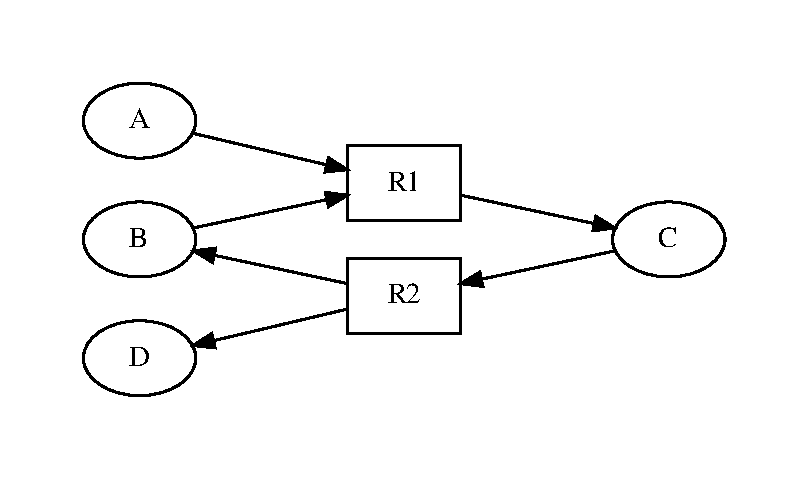
\includegraphics[width=0.6\textwidth]{reaction-network}
    \caption{The reaction network described by the chemical reaction equations \ref{eq:reaction-eqs} as a bipartite graph.}
    \label{fig:reaction-network}
\end{figure}

Given such a reaction network described by its reaction equations, 
we can also set up a \emph{stoichiometric matrix} $\mb{S} \in \mathbb{N}^{m \times n}$, 
where $m = |M|$ is the number of compounds present in the reaction network and $n = |R|$ the number of reactions in the network.
The entries $s_{ij}$ of $\mb{S}$ are then given as the difference of stoichiometric coefficients on the input and output sides 
of the $i$-th compound in the $j$-th reaction.
Note that sometimes the stoichiometric matrix is also defined as the transposed of $\mb{S}$.
For a general reaction equation with compounds $M = (M_1, M_2, \dots, M_m)^T$ and $n$ reactions
\begin{align}
    R_j: \sum_{i=1}^m k_{ij} M_i \to \sum_{i_1}^m \ell_{ij} M_i, \qquad \forall R_j \in R
\end{align}
the entries of the stoichiometric matrix therefore are $s_{ij} = k_{ij} - \ell_{ij}$.
The stoichiometric matrix for our exemplary reaction equations is given by
\begin{align}
    \mb{S} = \begin{pmatrix}
	-1 &  0 \\
	-1 &  1 \\
	1  & -1 \\
	0  &  1 \\
    \end{pmatrix}
\end{align}
Note that no catalystic effects can be described by the stoichiometric matrix, 
since the difference of left and right hand side stoichiometric coefficients will always cancel out catalysts.
%Reaction networks for organisms maybe found in the BioCyc database, the Kyoto Encyclopedia of Genes and 
%Genomes and other similar databases and repositories.

%The reaction network which we have described so far gives us a purely static view on our system.
%Consider to feed your system with some appropriate substrate, qualitatively you will not expect all of the metabolites to be present in the system at once.
%Instead the reactions associated with the incoming substrates will start turning it over into the metabolites specified by the corresponding reactions.
%It is therefore rather obvious that the reaction network so far does not carry any information about the dynamics of the system.
%The question rises at which rate this will happen and what metabolite concentrations will we be able to measure after some amount of time has passed.
%Determining these rates is the very goal of Metabolic Flux Analysis.

We now extend our formalism in order to take into account fluxes.
The fluxes we wish to determine are each associated with one of the reactions.
In the following we denote the fluxes as the vector $\mb{v}=(v_i, v_2, \dots, v_m)^T \in \mathbb{R}^m$, 
where $v_i$ is the reaction rate associated to reaction $R_i \in R$.
Under the assumption, that all metabolites are available plenty and reaction rates happen at a constant rate, 
we can define the time derivative of the metabolite concentration $\mb{x}=(x_1, \dots, x_n)^T$ where $x_i \in M$ as
\begin{align}
    \frac{\mathrm{d}}{\mathrm{d}t}\mb{x} = \mb{S}\mb{v}
\end{align}
which intuitively describes the rate of change of each metabolite as sum of the in and out fluxes.
By introducing the so-called steady state condition, we can restrict the space of possible fluxes to the solution of the linear system
\begin{align}
    \mb{S}\mb{v} = \mb{0} \label{eq:steady-state}
\end{align}
From a biological point of view the steady state condition puts the system into a metabolic steady state also known as homeostasis, 
where metabolite concentrations do not change anymore because the in and out fluxes cancel each other out.
In general, there exist more reactions than compounds in realisitic metabolic models \cite{noeh15, orth10}, 
i.e. $m > n$ which immediately leads to the linear system in \ref{eq:steady-state} to be underdetermined.
By the rank-nullity theorem, we have that the dimension of the null space of $\mb{S}$ is $k = \nullity(S) = m - \rank(S)$.
It follows that if we somehow determine $k$ linearily independent flux values, the rest can be computed from them as
\[
    \mb{v} = \mb{v}(\bomega) = \mb{K}\bomega
\]
where $\bomega \in \mathbb{R}^k$ are the \emph{free fluxes} and $\mb{K}$ is a basis of the nullspace of $\mb{S}$.

From a biological perspective, not every flux distribution $\mb{v}(\bomega) \in \Reals^m$ is biologically feasible or meaningful,
\eg upper limits on the absolute value or on the directionality of reactions may be known from thermodynamic considerations.
Also, usually the substrake uptake and other extracellular fluxes like $\mathrm{CO}_2$ production of the 
metabolism under consideration are directly measurable, allowing to fix their values or 
at least bound them within some narrow interval accounting for measurement noise. 
Taking these linear constraints of the form $\mb{\hat{A}}\mb{v} \leq \mb{b}$ into account, we obtain a convex polytope 
\begin{align}
    \mathcal{V} \coloneqq \big\{ \bomega \in \Reals^k : \mb{A}\bomega \leq \mb{b} \big\}
    \label{eq:convex-polytope}
\end{align}
with $\mb{A} \coloneqq \mb{\hat{A}}\mb{K}$, to which we will refer to as the \emph{flux polytope}.
In general, this flux polytope has a strictly positive volume, meaning that it usually does still not admit 
a unique solution to (\ref{eq:steady-state}).
%Taking these linear constraints of the form $\mb{A}\mb{v} \leq \mb{b}$ into account, we obtain a convex polytope 
%\begin{align}
%    \mathcal{V} \coloneqq \big\{ \bomega \in \Reals^k : \boldsymbol{\mathcal{A}}\bomega \leq \mb{b} \big\}
%\end{align}
%with $\boldsymbol{\mathcal{A}} \coloneqq \mb{A}\mb{K}$, to which we will refer to as the \emph{flux polytope}.

\subsection{Atom transition networks}
\label{sec:atom-transition-networks}

The technique of Flux Balance Analysis tries to obtain an unique flux distribution by assuming that the
organism under consideration has been optimized by evolution for some specific purpose e.g. growth or 
substrate uptake. 
These assumptions translate into linear objective functions on the flux polytope, 
reducing the problem of obtaining an unique flux distribution to an easy to solve linear program.
However the assumption made that the organism under consideration is optimized for some specific purpose
is very restrictive and may especially not apply when using unusual cultivation regimes or \emph{engineered}
organisms, which may never have felt the pressure of evolution.

Flux Balance Analysis does not need any measurement data at all but only the static reaction network,
whereas \Ciso Metabolic Flux Analysis on the other hand relies heavily on measurement data.
A naming property of \Ciso MFA is to obtain such measurements from \Ciso isotope labelling experiments.
Note that in general labellings are not restricted to carbon atoms only, but forming the basis of life on earth
and being the backbone of most biochemical molecules they are a very natural choice.
The input substrate gets labelled with \Ciso atoms at predetermined postitions and by time the labellings will be
distributed across the metabolites.
The labellings can then be measured using nuclear magnetic resonance (NMR) and mass spectrometry (MS).
In order to be able to use the isotope labelling experiment data, we need so called atom transition networks,
which as we will see will enable us to simulate isotope labelling experiments and hence lead to a naturally
arising residuum, which we can then aim to minimize.
Basic reaction networks usually map molecules to other molecules, atom transition networks concretize reactions 
on an atomic level, mapping the single atoms of the substract molecule
to the atoms in the product molecule by position.

\begin{figure}
    \centering
    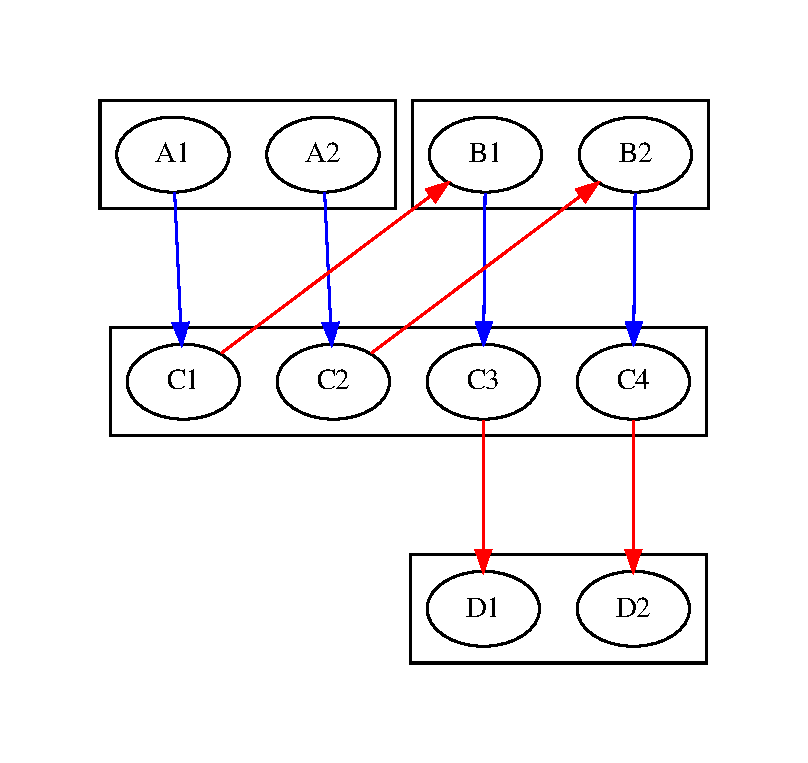
\includegraphics[width=0.6\textwidth]{atom-transition-network}
    \caption{
	Atom transition network of the toy example \ref{eq:reaction-eqs}. 
	Reactions are now color-encoded, blue stands for reaction $r_1$, red stands for reaction $r_2$.
    }
    \label{fig:atom-trans}
\end{figure}

\bigskip \noindent 
Let us reconsider our previous example reaction network and add some carbon atom information to the compounds 
as well as transition information to the reactions. 
Assume that the compounds $A, B$ and $D$ consist of two carbon atoms each and $C$ of four and consider the 
atom transitions as depictured in Figure \ref{fig:atom-trans}.
Similarily to Section \ref{sec:stoichiometric-modelling} we are interested in the rates of change of the now labelled metabolites.
Let $a_i, b_i, d_i$ and $c_k$ denote the different fractions of labeled metabolites $A, B, D$ and $C$ respectively, 
where $i=0,\dots,3$ and $k=0,\dots,15$ since every carbon atom can either be labelled or not, hence yielding 
a total of $2^\kappa$ possible different labelling states for every compound with $\kappa$ carbon atoms.
It is common to assume that the reactions on the isotopomer level follow a law of mass action, 
meaning that the reaction rates are proportional to the concentrations of the reactants.

Consider compound $C$ and in an abuse of notation let $C$ also denote the size of the metabolite pool.
Further let $\mb{v}=(v_1, v_2)^\top$ be a flux distribution to our two reaction toy example, 
then we get the following nonlinear differential equation
\begin{align}
    C \dv{t} c_k = v_1 a_i b_j - v_2 c_k, \qquad i,j=0,\dots,3, \quad k = 0, \dots, 15 
    \label{eq:exemplary-mass-bal}
\end{align}
yielding a total of 16 equations for compound C.
The nonlinear term $v_1 a_i b_j$ can be interpreted as the probability that a metabolite unit of the metabolite
pool $A$ in labelling state $i$ and a metabolite unit of the pool $B$ in the labelling state $j$ "hit" each other
and react scaled by the reaction rate~$v_1$. 
Similar equations to (\ref{eq:exemplary-mass-bal}) may be derived for all other metabolite pools $A, B$ and $D$,
which are then known as the \emph{mass balance equations}, which we denote as
\begin{align}
    \dv{t}\mb{y} = g(\mb{v}, t) \label{eq:mass-bal}
\end{align}
in the general case.
These equations form a dynamic system of nonlinear ordinary differential equations, 
which has been proven to always converge towards a unique equilibrium \cite{wiechert01}
\begin{align}
    \dv{t} \mb{y} = g(\mb{v}, t) = 0 \label{eq:nonlin-sys}
\end{align}
where $\mb{y} \in I$ is the vector of all isotopomers of every metabolite in the system 
and we denote the isotop labelling space $I \subset \Reals^\eta$, where 
\[
    \eta = \sum_i^m 2^{\kappa_i}
\]
where $\kappa_i$ is the number of carbon atoms in metabolite $M_i$.
The condition (\ref{eq:nonlin-sys}) describes the so called \emph{isotopic steady state}.
Notice that the pool sizes as \eg given in the differential equation (\ref{eq:exemplary-mass-bal})
are constant since we consider the metabolic steady state.
Hence the pool sizes vanish in equation (\ref{eq:nonlin-sys})
Given an atom transition network, an input substrate labelling and a flux distribution, 
we are now able to perform simulations of labelling data.

\subsection{Forward simulations}
\label{sec:forward-simulations}

Let $\ffp = \big\{ \mb{K}\bomega : \bomega \in \fp \big\}$ be the space of all feasible flux distributions.
Forward simulations in \Ciso MFA are maps $f: \ffp \times [0,\infty] \to \is$ from the feasible flux space $\ffp$
and a given time $t \in [0,\infty]$ to the isotope labelling space $\is$. 
If a flux distribution $\mb{v} \in \ffp$ is given, then the forward 
simulation allows us to predict isotope labelling values at any time $t \in [0,\infty]$ and to 
compare the result with actual measurements to assess the quality of our flux distribution $\mb{v}$.
In the following we denote $\mb{y} = f(\mb{v}, t) \in \is$. 
%For steady-state scenarios, \ie scenarios where we assume the organism to reside
%in a metabolic steady state also known as homeostasis, a forward simulation can be computed by solving the
For isotopic steady-state scenarios, we set $t=\infty$ and write $\mb{y} = f(\mb{v}, \infty) = f(\mb{v})$,
which is why we included $\infty$ explicitly in the previous definition of $f$.
A forward simulation can then be computed by solving the algebraic system 
\[
    \dv{t}\mb{y} = \dv{t}f(\mb{v}) = g(\mb{v}, t) = 0
\]
where $\dv*{\mb{y}}{t}$ are the time derivatives of the isotope labellings, given by 
the mass balance equations $g(\mb{v},t)$ defined as in Equation \ref{eq:mass-bal}.
As stated before, this nonlinear system admits a unique solution for the kind of problems which we are dealing here \cite{wiechert01}.

For instationary scenarios, \ie problems where the real measurements where taken before the isotopically 
steady state was reached, the measurements are complemented with timestamps of the measurement. 
Hence, to obtain a forward simulation at the particular time $t_0$ of a measurement, 
the time derivatives have to be integrated up the desired time $t_0$ to obtain 
\[
    \mb{y}(t_0) = \int_0^{t_0} g(\mb{v},t) \dd{t}
\]
which is the isotope labelling data predicted at time $t_0$.

Since, as discussed before, the flux distribution is uniquely determined by the $k$ free fluxes $\bomega$,
we can defined $\mb{y}$ also as a function of the free fluxes, \ie
\[
    \mb{y}(t) = f(\mb{K}\bomega, t)
\]
which abusing notation we will from here on also simply denote as $\mb{y}(t) = f(\bomega,t)$.

\subsection{Estimating flux distributions}
\label{sec:estimating-flux-distributions}

Now that we are equipped with the ability to simulate isotope labelling experiments, 
suppose we are given an isotope labelling measurement $\bmu$ and its respective timestamp $t_{\bmu}$.
Intuitively speaking, we want to assess if the simulated measurements will be close to the actual
measurements using a given flux dsitribution $\mb{v}(\bomega)$.
%\hyphenation{mea-sure-ments} using a given flux dsitribution.
If we now pick an arbitrary flux distribution $\bomega$ from our flux polytope $\fp$, 
we can perform the forward simulation and receive a measurement prediction ${\mb{y} = f(\bomega, t_{\bmu})} = f(\bomega)$,
where we use the latter as a short hand notation when $t_{\bmu}$ is clear from context.
By taking the sum of squares residual
\begin{align}
    r_{\bmu} ( \bomega ) \,=\, \big\| f(\bomega) - \bmu \big\|_{\mb{\Sigma}^{-1}}^2
			\,=\, \big\| \mb{y} - \bmu \big\|_{\mb{\Sigma}^{-1}}^2 
			\,=\, \big( \mb{y} - \bmu \big)^\top \mb{\Sigma}^{-1} \big( \mb{y} - \bmu \big)
    \label{eq:ssr} 
    \\[-12pt] \nonumber
\end{align}
we obtain a measure for the quality of our flux distribution, where $\mb{\Sigma}$ contains the squared
standard errors of the measurements on the diagional axis.
Since measurements may be assumed to be independent from each other, $\mb{\Sigma}$ is diagonal in our case
and computing the inverse is trivial.
The problem
\begin{align}
    \bomega^* = \arg\min_{\bomega \in \fp} \, r_{\bmu} ( \bomega )
\end{align}
is equivalent to the maximum likelihood estimation problem, if we consider the sum of~squares
residual as proportional to the negative log-likelihood.
Such point estimators have to be considered with caution as the measurement data we are provided 
comes with measurement noise for which a point estimator cannot come up for.
Intuitively speaking, the maximum likelihood estimator provides us the flux most likely to explain
the data, assuming the data is correct.
This being said, it is a natural goal to quantify the uncertainity introduced by the noise as well.
Bayesian statistics, which have been on the rise in the last decades, give us an intuitive way of quantifying
the uncertainity related to various issues, that are found within our modelling approach.
%A problem which arises with such point estimators is the lack of information 
%Our goal is basically to minimize $\epsilon_{\bmu}(\mb{v})$.
%However this target function $\epsilon_{\bmu}(\mb{v})$ is highly nonlinear and may have several
%optima.

In a Bayesian framework, we are interested in the \emph{posterior distribution} $\Pr(\bomega|\bmu)$ 
which gives us the probability of a parameter based on the data. 
From Bayes' Theorem follows that we can compute this posterior distribution as 
%\begin{align} 
%    \Pr(\bomega|\bmu) = \frac{ \Pr(\bmu|\bomega) \Pr(\bomega) }{ \Pr(\bmu) } \propto \Pr(\bmu|\bomega) \Pr(\bomega) 
%\end{align} 
\begin{align} 
    \nonumber \\[-12pt]
    \Pr(\bomega|\bmu) = \frac{ \Pr(\bmu|\bomega) \Pr(\bomega) }{ \Pr(\bmu) } \propto \Pr(\bmu|\bomega) \Pr(\bomega) 
    \label{eq:posterior}
    \\[-12pt] \nonumber
\end{align} 
where $\Pr(\bmu|\bomega)$ is the \emph{likelihood function} and $\Pr(\bomega)$ is our \emph{prior} belief.
In our case, this prior belief is that the flux distribution should lie inside the flux polytope $\fp$, 
\ie 
\begin{align} 
    \Pr(\bomega) = \begin{cases}
	\varphi & \text{if } \bomega \in \fp \\
	0 & \text{else}
    \end{cases}
    \label{eq:prior}
\end{align} 
but since any of these flux distributions seems equally likely \emph{a priori} we choose 
$\varphi$ such that $\int_{\fp} \Pr(\bomega) \dd\bomega = 1$.
In words, we assume that the flux distribution is uniformly distributed within $\fp$.
The likelihood function is a model which relates the unknown parameters and the given data.
Intuitively speaking it translates how likely it would be to observe the outcome of the data $\mu$
given that $\bomega$ where the true parameters.
A common choice is to assume that measurements are normally distributed, resulting in the likelihood function
\begin{align}
    \nonumber \\[-12pt]
    \Pr(\bmu|\bomega)	= \frac{1}{Z}\exp{{-\frac{1}{2}r_{\bmu}(\bomega)}} 
    = \frac{1}{Z}\exp{{-\frac{1}{2}\big( f(\bomega, t_{\bmu}) - \bmu \big)^\top \mb{\Sigma}^{-1} \big( f(\bomega, t_{\bmu}) - \bmu \big)}}
    \label{eq:likelihood}
    \\[-12pt] \nonumber
\end{align}
where ${Z=\sqrt{(2\pi)^\eta\det\Sigma}}$ and $m$ is the dimension of the isotope labelling space. 
To point out that the likelihood function is a function of the parameter vector $\bomega$ and not of the measurement $\bmu$,
we denote it also as $\likeli_{\bmu}(\bomega) \coloneqq \Pr(\bmu|\bomega)$.
Note that the likelihood function in (\ref{eq:likelihood}) is not a closed-form expression, 
since $f$ requires computation of either an algebraic system of equations or an integral.
Also, it is therefore not possible to directly draw samples from this distribution. 
Instead such problems are tackled by employing Markov Chain Monte Carlo algorithms.
The key idea is to construct a Markov Chain, whose stationary distribution converges to the desired target function.
Some key concepts and the derivation of the particular Markov chain for our purposes are given in the following section.

\subsection{Markov chain Monte Carlo algorithms}

A Markov chain is a stochastic process $(X_n)_{n \geq 0}$ on a state space $S$, which is defined by a starting 
distribution $\lambda$ and a transition kernel $\tk: S \times S \to [0, 1]$, for which
\[
    \sum_{j \in S} \tk(i,j) = 1, \quad \forall i \in S
\]
holds and which contains the transition probabilities, \ie
\[
    \Pr(X_{n+1} = j | X_{n} = i, X_{n-1} = x_{n-1}, \dots, X_0 = x_0) = \tk(i,j)
\]
which intuitively means that the transition probability from the state at time $n$~to~${n+1}$ does
not dependent on the chains history before $n$.
A distribution $\pi: S \to [0,1]$ is said to be an \emph{invariant} or \emph{stationary measure} 
of $\tk$, if 
\[
    \pi \tk = \pi \quad \Leftrightarrow \quad \sum_{i \in S} \pi(i)\tk(i,j) = \pi(j) %= \pi(j) \underbrace{\sum_{i \in S} \tk(i, j)}_{=1}
\]
and \emph{invariant} or \emph{stationary distribution} if also 
$\sum_{i \in S} \pi(i) = 1$ holds.
A sufficient condition for $\pi$ to be invariant, is 
\begin{align}
    \pi(i) \tk(i,j) &= \pi(j) \tk(j,i) \label{eq:detailed-balance} 
\end{align}
which is widely known as the \emph{detailed balance condition}.
Assuming detailed balance and taking the sum over $i \in S$ on both sides we obtain
\[
    \sum_{i \in S} \pi(i) \tk(i,j) \, = \, \sum_{i \in S} \pi(j) \tk(j,i) \, = \, \pi(j) \sum_{i \in S} \tk(j,i) \, = \, \pi(j)
\]
which shows that $\pi$ indeed is invariant under $\tk$.
Our goal in order to approximate the posterior distribution $\Pr(\bomega|\bmu)$ is to construct 
a Markov chain such that it has $\Pr(\bomega|\bmu)$ as its unique invariant distribution, 
to which the detailed balance equation is a key concept.
Hastings \cite{hastings70} made the following ansatz, 
\[
    \tk(i,j) \coloneqq \begin{cases}
	p(i,j)a(i,j) & \text{if } i \neq j \\[3mm]
	1 - \sum\limits_{k \neq i} \, p(i,k)a(i,k) & \text{if } i = j
    \end{cases}
\]
where $p(i,j)$ is the \emph{proposal distribution} and $a(i,j)$ the \emph{acceptance probability}.
Note that detailed balance holds trivially for $\tk(i,i)$.
Plugging the ansatz for $i\neq j$ into the the detailed balance equation, we obtain
\[
    \pi(i)p(i,j)a(i,j) = \pi(j)p(j,i)a(j,i) \quad \iff \quad \frac{a(i,j)}{a(j,i)} = \frac{\pi(j)p(j,i)}{\pi(i)p(i,j)}
\]
where using the \emph{Metropolis criterion} 
\begin{align}
    a(i,j) \coloneqq \min\bigg\{ 1, \frac{\pi(j)p(j,i)}{\pi(i)p(i,j)} \bigg\} 
    \label{eq:metropolis}
\end{align}
indeed satisfies detailed balance.
The distribution for which we want to generate samples is our posterior distribution as defined in (\ref{eq:posterior}) 
and hence for $\bomega_n \in \fp$ we obtain the Metropolis criterion for our Markov chain as
\begin{align}
    \nonumber \\[-12pt] 
    a(\bomega_n,\bomega_{n+1}) 
	&= \min\bigg\{ 1, \frac{ 
	    \Pr(\bomega_{n+1}|\bmu) \, p(\bomega_{n+1}, \bomega_n) 
	}{ 
	    \Pr(\bomega_n|\bmu) \, p(\bomega_n, \bomega_{n+1}) 
	} \bigg\} 
	\nonumber \\[2mm]
	&= \min\bigg\{ 1, \frac{ 
	    \likeli_{\bmu}(\bomega_{n+1}) \, p(\bomega_{n+1}, \bomega_n) 
	}{ 
	    \likeli_{\bmu}(\bomega_n) \, p(\bomega_n, \bomega_{n+1}) 
	} \bigg\}
	\label{eq:bayes-metropolis}
    \\[-12pt] \nonumber
\end{align}
We remark some convenient properties of the Metropolis criterion.
The normalization constant $\Pr(\bmu)$, the prior $\Pr(\bomega)\big|_{\fp} = \varphi$ as well as the constant $Z$ 
introduced in (\ref{eq:likelihood}) are cancelled out here. 
This is especially interesting as we avoid explicit computation of the high-dimensional integrals
\begin{align}
    \nonumber \\[-12pt] 
    \Pr(\bmu) = \int_{\fp} \Pr(\bmu|\bomega)\Pr(\bomega)\dd\bomega
    \qquad \text{and} \qquad
    \Pr(\bomega) \Big|_{\fp} = \varphi = \frac{1}{\int_{\fp} \dd \bomega}
    %\\[-12pt] \nonumber  
\end{align}
However note that every evaluation of the Metropolis criterion (\ref{eq:bayes-metropolis}) 
requires performing a forward simulation in order to compute the likelihood function 
$\likeli_{\bmu}(\bomega_{n+1})$, even for moves that might be rejected, which is an issue we 
will revisit later.
In general, our Metropolis criterion (\ref{eq:bayes-metropolis}) becomes undefined for $\bomega_n \notin \fp$ 
as then $\Pr(\bomega_n)=0$ (\cf (\ref{eq:prior})). 
Assuming that $\bomega_n \in \fp$ however, we have that for every $\bomega_{n+1} \notin \fp$, 
\[
    \Pr(\bomega_{n+1}) = 0 \quad \implies \quad a(\bomega_n, \bomega_{n+1}) = 0
\]
and hence if we require 
\[ 
    \supp(\lambda) \subseteq \fp 
\] 
for our starting distribution $\lambda$, meaning
that we will definitely start the Markov chain inside our parameter space $\fp$, 
we can guarantee that it will never escape from $\fp$.
More formally, any \emph{closed communicating classes} of our Markov chain will lie within $\fp$, where we refrain
from giving precise definitions and instead refer to \cite{norris97}.

A Markov chain is said to be \emph{irreducible}, if its state space forms on single closed communicating class, 
which basically means that every state is reachable from every other state in a finite number of steps. 
If a Markov chain is irreducible, then its invariant measure is unique up to scaling. 
%However, this does not necessarily mean that there also exists an invariant distribution, as normalizing the
%measure requires the integral over the measure to converge.
%More formally, we obtain an invariant distribution $\hat{\pi}$ from an invariant measure $\pi$ as
%\[
%    \hat{\pi}(i) = \frac{\pi(i)}{\sum_{j \in S}\pi(j)}
%\]
%which is only well-defined, if $\sum_{j \in S}\pi(j) < \infty$. 
%In our case however, because our state space is finite \wrt to the Lebesgue measure, existence of an invariant
%distribution is indeed guaranteed.
Irreducibility is achieved by using an appropriate proposal distribution.
In fact proposal distributions that satisfy irreducibility are easily obtained and most naive approaches will
do so out of the box.
In the following we quickly present some frequently used proposal distributions along with their strengths
and weaknesses.

%An important property of a Markov chain is its so called \emph{mixing time}, which is the number of samples needed
%until the generated distribution is \emph{close} to the target distribution \wrt some appropriate distance measure.
%Without dwelving into a more formal introduction to the topic, we remark that our goal is to have small mixing 
%times in order to converge quickly.

\subsubsection{Proposal distributions}

\todo{quickliy present a hand full of proposal distributions and issues with rejection-based moves} 

\paragraph{Ball Walk}
The ball walk uniformly picks a point $y$ from the $k$-dimensional ball $\mathcal{B}$ with radius $\delta$ and 
midpoint $x$, which is our current state. If $y$ lies outside $\fp$, which can happen when 
$\mathcal{B} \cap \fp \neq \emptyset$, the move gets automatically rejected.
If $y \in \fp$, then the move gets accepted or rejected with probability $a(x, y)$, where $a(\cdot, \cdot)$ is 
the Metropolis criterion from (\ref{eq:bayes-metropolis}).

This proposal move is in a sense rejection based as it does not take into account the structure
of the state space $\fp$ at all and creates infeasible moves.
In an unfortunate situation, \eg when $x$ sits close to the boundaries in a pointy corner of a high-dimensional
poltyope, the fraction of $\mathcal{B}$ which lies outside $\fp$ can be vast hence also most probably leading 
to a vast number of infeasible proposals.
This problem is especially striking in high dimensions and very much comparable to the phenomenon of the 
ratio of the volume of an inscibed hypersphere to the volume of a hypercube exponentially decaying to zero
as dimensions increase.

\paragraph{Hit and Run}

Hit-and-Run proposals ''shoot'' a chord from its current position $\mb{x}$ into some uniformly randomly picked 
direction $\mb{d}$ and move along this chord $\mb{y} = mb{x} + \alpha\mb{d}$.
The size of the step $\alpha$ can be controlled by controlling the distribution with which a point along the ray is picked.
Apart from using an uniform distribution on the chord, one can also choose an one-dimensional normal distribution with 
the current state as mean.
This will promote shorter steps, which usually contain less risk of being rejected at the cost of being more
correlated and thus resulting in less statiscal efficiency.
Note that computing the intersections of the chord $\mb{x} + \alpha \mb{d}$ with the boundaries of the polytope
can be easily achieved by taking the minimal and maximal values from the vector
\[
    \frac{\mb{b} - \mb{A}\mb{x}}{\mb{A}\mb{d}}
\]
for the parameter $\alpha$, where the fraction denotes an elementwise fraction and $\mb{A}$ and $\mb{b}$ 
describe the linear constraints of our polytope $\fp$ as in (\ref{eq:convex-polytope}).

\paragraph{Dikin Walk}



\paragraph{CSmMALA}

\subsection{The challenge}

In general, the process of solving the inverse problem of estimating flux distributions using Markov chain Monte Carlo
algorithms is well-defined.
One major difficulty however is the usage of isotopically instationary measurements within this framework, 
because, as we mentioned before, every step of the Markov chain requires an evaluation of the forward simulation.
For isotopically instationary scenarios, this forward simulation turns into the problem of numerically integrating 
a system of ordinary differential equations, which for some flux distributions turns into a \emph{stiff} problem.
Although numerical solutions to ordinary differential equations are a well-investigated topic, in the presence of stiff
problems the simulation time can go up significantly \todo{\cite{?}}, making flux estimation in isotopicaly instationary
scenarios expensive.
Obviously speeding up forward simulations would be a natural target, however regarding the long presence of 
numerical solvers for ordinary differential equation and the fact that dedicated work has already been put into
accelerating solvers and methods for ordinary differential equations derived from reaction networks \cite{stratmann19},
this approach does not appear too fruitful.

Another approach, on which we will focus within this expos\'e is to instead reduce the number of forward simulations needed.

\bigskip
\noindent \todo{from here on still very much a draft}
\bigskip

One possible way to avoid its evaluation is to approximate its value e.g. by using regression
models. 
The natural question, which arises is on what data to fit the regression model.
Creating samples is not only costly, but the samples need to represent the true underlying function
and hence would have to be taken from a convergent Markov chain.
This again contradicts our goal to run exactly such a Markov chain using the regression model.

On the other hand, computing approximate models online, i.e. while sampling, would violate the fundamental Markov property
destroying the theoretical basis for the convergence of our chain.
The field of adaptive Markov chains deals with this issue, where the proposal distribution is adapted online
from the chains history, but in a fashion that keeps convergence guaranteed.


\section{Multifidelity methods}
\label{sec:multifidelity}

\subsection{Reduced networks from reduced measurements}
Reduce networks by reducing measurements and hence omit metabolites which do not affect the measured pools at all.
Less measurements however lead to fluxes, which are only found in the backtrace of the omitted 
measurements to become structurally non-identifiable.
The question arises how many measurements should be omitted to obtain a good tradeoff between 
computational cost and drawbacks from increased non-identifiabilities.
It has to be investigated more closely how non-identifiabilities propagate and what effect they
have on the adapted proposal step using the low-fidelity model.

Identifying the reduction in size of the network from omitting measurements is most probably 
feasible.
Doing so allows to control speedup and degree of non-identifiability introduced.

\subsection{Stationary and instationary scenarios}
Combine stationary and instationary scenarios, where stationary scenarios act as low-fidelity method. 
Often only one or the other is available from an isotope labelling experiment. 
Stationary values however might be extrapolated using time-series analysis from instationary data. 
    
\subsection{Regression models on pre-run data}
Pre-runs allow to generate data points from the posterior distribution on which approximate models can
be computed.
Such pre-runs will not be run until convergence as this would make any follow up run superfluous.
Therefore the samples produced will have no guarantee of being distributed according to the posterior distribution.
This means, close to samples of the pre-runs the approximate model will reflect the function $\likeli_{\bmu}(\bomega)$
quite well, further away arbitrary large errors might be introduced.

\cite{muller20} propose to use a trust criterion where the approximate model is not used if moves got rejected more
than $N$ times in a row and used again if $M$ moves got accepted in a row using the accurate MALA proposal step.
In the case where the approximate model is distrusted, the $N$ rejected moves get removed from the set of samples.
\cite{muller20}  do not use their approach in a multifidelity framework but in an alternating manner.
The multifidelity method using an intermediate low-fidelity step if the approximate model is trusted and no
intermediate step if the approximate model is currently distrusted can be seen as two different transition
kernels which have the same stationary distribution as a target distribution but are used mixed.
It seems provable that this mixed usage of these transition kernels is permitive under mild conditions such
as irreducibility of both transition kernels and given that a low-fidelity approximation may be arbitrarily bad
without threatening convergence.

Gaussian process regression delivers standard deviation intervals at every evaluated point and hence is 
basically already shipped with a natural trust criterion, where one can for example set a hard threshold on which to
decoed if the model is used or not.
Also it could be randomly decided whether the regression model is used or not with probability proportional to the 
precision of the estimate.

\subsection{Combination with multistage approaches}

The cheap evaluation of coarse model functions also allows for delayed-rejection schemes, where a proposal
rejected by the coarse model can be corrected a few times before being assessed by the high-fidelity model.
These stacked proposal corrections are even allowed to use the previously rejected proposals in order to 
optimize the current proposal. 
In the end however a single new sample is produced and hence too many corrections may increase computational
cost over what is sensible to actually decrease overall computational costs.

\subsection{Theoretical considerations}

What conditions do low-fidelity models have to meet to actually allow for convergence?
It might well be that low-fidelity models are allowed to be arbitrarily bad without threatening
theoretical convergence properties at least if some basic properties like irreducibility are maintained.
Results in \cite{efendiev06} hint that the support of the target distribution being contained 
in the support of the low-fidelity model is a sufficient condition.
In practice low-fidelity models with large approximation errors will most likely lead to a
reduction of computational efficiency. 
What conditions should be met to allow for an increase of computational efficiency?
Probably conserving monotonicity properties might be a promising condition, since this will lead
to a bias in the proposal moves somewhat proportional to the acceptance probability of the accurate
model.

\bigskip
\noindent \todo{from here on still very much a draft}
\bigskip

Multi-Stage (or apparently also sometimes called Delayed-Acceptance/Rejection) algorithms 
use differently costly forward simulations cascaded after each other [4,5].
The idea is to quickly compute a coarse value as an approximate to the finer ones and only
consider promising looking areas.
A first proposal is accepted or not using the energy function of the coarse simulation result and 
only if the move gets accepted by the first stage the next finer simulation is evaluated.
This saves costly computations of exact solutions for proposal steps which might have been rejected
anyway.

The natural questions which arises here is what kind of coarse and fine versions of the model 
functions to apply.
In our case, where a forward simulation consist of solving a system of nonlinear ordinary differential 
equations using numerical integration a natural choice would be the integration step size or - when using
adaptive schemes - the error tolerance.
In particular, one could arange a sequence of different error tolerances where each proposal stage
solves the system again using a lower tolerance.
According to [3], a decrease of accuracy from 1e-3 to 1e-9 might lead to an increase in computational
time taken in an order of magnitude.

Further choices, which are more closely related to our domain, would be stationary and instationary 
measurements, which would form coarse and fine model respectively.
However often this data is not available in mixed form, meaning that a isotope labelling experiment
only either contains measures from the stationary or instationary phase of the experiment.

Also, MS measurements are easier to simulate than MS-MS measurements, hence one could also apply
a two-stage proposal scheme here.

Another, again more general approach, is the application of linear or higher order models to 
approximate the function at least locally.
The question arises what data to use to setup such models.
Evaluation of the gradient locally is expensive in general, since it needs exact evaluations of
the forward simulation.
Such evaluations are obviously available from the previous samples.
However, using this data to obtain a model of the forward simulation, we would violate the Markov
property.

[2] proposed a method where gradient evaluations are taken from a neural network trained on a pre-run of
the chain.
The approximate evaluations are used within some trust-criteria, meaning that as soon as one starts
to distrust the approximation (e.g. because to many rejections happened), the exact evaluation is used
again and as soon as the approximation has matched the exact evaluation well enough, one switches back
to using the approximation.
The overall concept can most probably be used with any approximate model of the gradient, not necessarily
a neural network, but for instance regression models applied to the prerun data.

An issue one might encounter using this approach, is that a model fitted on a prerun of a chain,
which did not run until convergence, may fail to approximate the target function well in some non-covered areas.
Although precautions are taken above, by not solely relying on the model, but only within trust criteria,
this may obstruct convergence to the correct target function.


\section{Adaptive Markov Chains}

The previous point about using online models fitted on the chains data leads to the broad field of Adaptive MCMC 
methods, which enable usage of the chains history to tune the proposal distribution s.t. less proposals get rejected,
but sill the whole chain remains convergent.



\section{Active Subspaces}

Informally speaking, active subspace methods try to identify the subspaces of the parameter space which explain 
most of the variation of some target function $g: U \to \Reals$, with $U \subset \Reals^n$. 
I presume, that they can also be considered as performing a principal component analysis on the samples generated 
by a chain and hence identifying the dimensions which explain most of the variance in the data.
The value in this information lies in the fact, that a direction, along which the target function does not (or only
minimally) change might not be worth exploring at all, since no information can be gained.
Parameters, for which its partial derivative is zero over the whole domain, are called non-identifiable.
In the case, where the active subspace may not be parallel to any parameter axes, a basis transformation towards
an orthogonal basis (like the eigenbasis) might be considered, yielding linear combinations of non-identifiable 
paramters.

The information on the active subspaces could either be collected and used in an offline or online fashion, again meaning
that one either tries to gain this information a priori using e.g. preruns of the chain or other techniques, 
or on the other hand by computing it while running the Markov chain and integrate the gained knowledge in an adaptive way,
s.t. convergence may still be guaranteed.



\section{Action Plan}

As a starter, an easy and straight-forward strategy could be to consider, implement and test the multi-stage MCMC method
using different error thresholds for the adaptive ODE solver as a first proof of concept. 
Careful software design could enable us to replace the coarse/fine models with arbitrary ones, allowing us to test
more combinations from what was mentioned previously.

Preconditioning of MCMC methods using a priori computed data like active subspaces and approximate models combined with
the trust criterion approach used in [1] also seem like a powerful, but rather simply implemented approach. 
Using approximate models of the function to cheaply evaluate its gradient could also be used to improve computational
efficiency of gradient-based approaches like the CSmMALA proposal move.
However, this most likely seems to remain compatible with the multi-stage approach, possibly allowing again for arbitrary 
combinations of techniques.

Generally, I consider the techniques above very powerful, since they work on a meta~plane above the considerations of efficient proposal distributions on convex polytopes. 
This \hyphenation{allows} to consider the techniques more as a framework, where arbitrary proposal moves, which suffice our needs, may be used.

The true excitement however obviously lies in the field of the adaptive methods, which however might leave the scope of 
a Master Thesis, considering the broad possiblities already outlined before.


%\bibliographystyle{ieeetr}
%\bibliographystyle{acm}
\bibliographystyle{siam}
\bibliography{literature}

\end{document}


